\documentclass{article}
\usepackage{graphicx}
\usepackage{fancyhdr}
\usepackage{setspace}
\usepackage{array}
\usepackage{hyperref}
\usepackage{ragged2e}
\hypersetup{hidelinks}

\onehalfspacing
\pagestyle{fancy}
\fancyhf{}

\fancyhead[L]{\small \textbf{Software Requirement Specification for AI-Driven Optimization of Local Body and MP Fund Management}}
\fancyfoot[C]{\thepage}

\title{\textbf{Software Requirement Specification} \\
\textbf{AI-Driven Optimization of Local Body and MP Fund Management} \\
\begin{center}
  \textbf{Prepared by} \\[0.5cm]
Paul Binu  (MAC22CD048)\\
Paulu Wilson (MAC22CD049)\\
Ronal Shoey George (MAC22CD051) 
  
 
\end{center}}

\begin{document}

\maketitle
\newpage

\tableofcontents 
\newpage

\section{Introduction}
\subsection{Purpose}
This document provides a detailed description of the AI-driven web application for optimizing Local Body and MP fund management. It outlines the purpose, key functionalities, and system requirements to ensure equitable fund allocation, real-time monitoring, and enhanced transparency using AI/ML.

\subsection{Document Conventions}
The document follows these formatting conventions:
\begin{itemize}
    \item Headings: \textbf{Bold}
    \item Sub-Headings: \textit{Italicized}
    \item Normal Text: Regular
\end{itemize}

\subsection{Intended Audience and Reading Suggestions}
This SRS is intended for:
\begin{itemize}
    \item Developers and AI engineers
    \item Government policy makers
    \item Project stakeholders and evaluators
    \item End-users (local government officials, auditors)
\end{itemize}

\subsection{Product Scope}
The system provides AI-powered analytics for fund allocation, project prioritization, fraud detection, real-time monitoring, and public engagement. It supports:
\begin{itemize}
    \item \textbf{AI-driven fund allocation} based on socio-economic data.
    \item \textbf{Project prioritization} using NLP-based sentiment analysis of community feedback.
    \item \textbf{Fraud detection} through anomaly detection and blockchain-based tracking.
    \item \textbf{Real-time project tracking} via IoT and satellite imagery.
    \item \textbf{Public engagement} using chatbots and AI-driven recommendation systems.
\end{itemize}

\subsection{References}
\begin{itemize}
    \item Government fund management guidelines
    \item Research papers on AI in governance
    \item Best practices in financial technology and data analytics
\end{itemize}

\newpage
\section{Overall Description}
\subsection{Product Perspective}
The system is a web application that integrates machine learning, NLP, and real-time monitoring to optimize fund utilization and governance transparency.

\subsection{Product Functions}
\begin{itemize}
    \item Fund allocation optimization
    \item Project prioritization using AI/ML
    \item Real-time fraud detection and compliance monitoring
    \item Public sentiment analysis and engagement
    \item Automated impact assessment
\end{itemize}

\subsection{User Classes and Characteristics}
\begin{itemize}
    \item \textbf{Government Officials} – Manage fund allocation and project approvals.
    \item \textbf{Auditors \& Analysts} – Monitor fund usage and detect anomalies.
    \item \textbf{General Public} – Provide feedback on projects.
    \item \textbf{Developers \& Data Scientists} – Maintain AI models and infrastructure.
\end{itemize}

\subsection{Operating Environment}
\begin{itemize}
    \item Web-based system accessible via modern browsers.
    \item Cloud-based deployment with AI-driven backend.
    \item Secure data storage and processing.
\end{itemize}

\subsection{Design and Implementation Constraints}
\begin{itemize}
    \item Compliance with government data security policies.
    \item Integration with existing fund management systems.
    \item Scalability to support nationwide implementation.
\end{itemize}

\subsection{User Documentation}
\begin{itemize}
    \item Online help center.
    \item User manuals for officials and stakeholders.
    \item API documentation for developers.
\end{itemize}

\subsection{Assumptions and Dependencies}
\begin{itemize}
    \item Reliable internet connectivity.
    \item Availability of structured government fund allocation data.
    \item Support from government bodies for implementation.
\end{itemize}

\newpage
\section{External Interface Requirements}
\subsection{User Interfaces}
\begin{itemize}
    \item Web dashboard for fund allocation and project monitoring.
    \item Chatbot interface for public engagement.
    \item Visual analytics for fraud detection and compliance.
\end{itemize}

\subsection{Hardware Interfaces}
\begin{itemize}
    \item Server infrastructure to support AI processing.
    \item IoT and satellite-based tracking for project monitoring.
\end{itemize}

\subsection{Software Interfaces}
\begin{itemize}
    \item Backend: Python (Django/Flask)
    \item Frontend: React.js / HTML, CSS
    \item Database: PostgreSQL / MongoDB
    \item AI Models: TensorFlow / PyTorch
    \item NLP: Hugging Face Transformers
    \item Blockchain: Hyperledger Fabric
\end{itemize}

\subsection{Communication Interfaces}
\begin{itemize}
    \item Secure HTTPS protocol for data transfer.
    \item API integrations with government databases.
\end{itemize}

\newpage
\section{System Features}
\subsection{Fund Allocation Optimization}
\begin{itemize}
    \item AI-driven predictions for fund distribution.
    \item Clustering algorithms for region-based prioritization.
    \item Optimization models for impact maximization.
\end{itemize}

\subsection{Project Prioritization}
\begin{itemize}
    \item NLP-based analysis of community feedback.
    \item Multi-criteria decision-making models for project ranking.
\end{itemize}

\newpage
\section{Other Nonfunctional Requirements}
\subsection{Performance Requirements}
\begin{itemize}
    \item Quick response time for AI predictions.
    \item Scalable cloud-based architecture.
\end{itemize}

\subsection{Security Requirements}
\begin{itemize}
    \item End-to-end encryption for sensitive data.
    \item Role-based access control for officials and auditors.
\end{itemize}

\subsection{Software Quality Attributes}
\begin{itemize}
    \item \textbf{Reliability} – Robust AI models for consistent predictions.
    \item \textbf{Maintainability} – Modular architecture for easy updates.
    \item \textbf{Portability} – Compatible across various devices and browsers.
    \item \textbf{Scalability} – Designed to handle large-scale government data.
\end{itemize}

\newpage
\section{Appendices}
\subsection{Appendix A: Glossary}
\begin{itemize}
    \item \textbf{Drug Repurposing}: Finding new uses for existing drugs.
    \item \textbf{SRS}: Software Requirement Specification.
    \item \textbf{HDGAT}: Heterogeneous Drug-Disease Graph Attention Network.
\end{itemize}

\subsection{Appendix B: Analysis Models}
\begin{itemize}
    \item Flow Diagram.


    \centering
    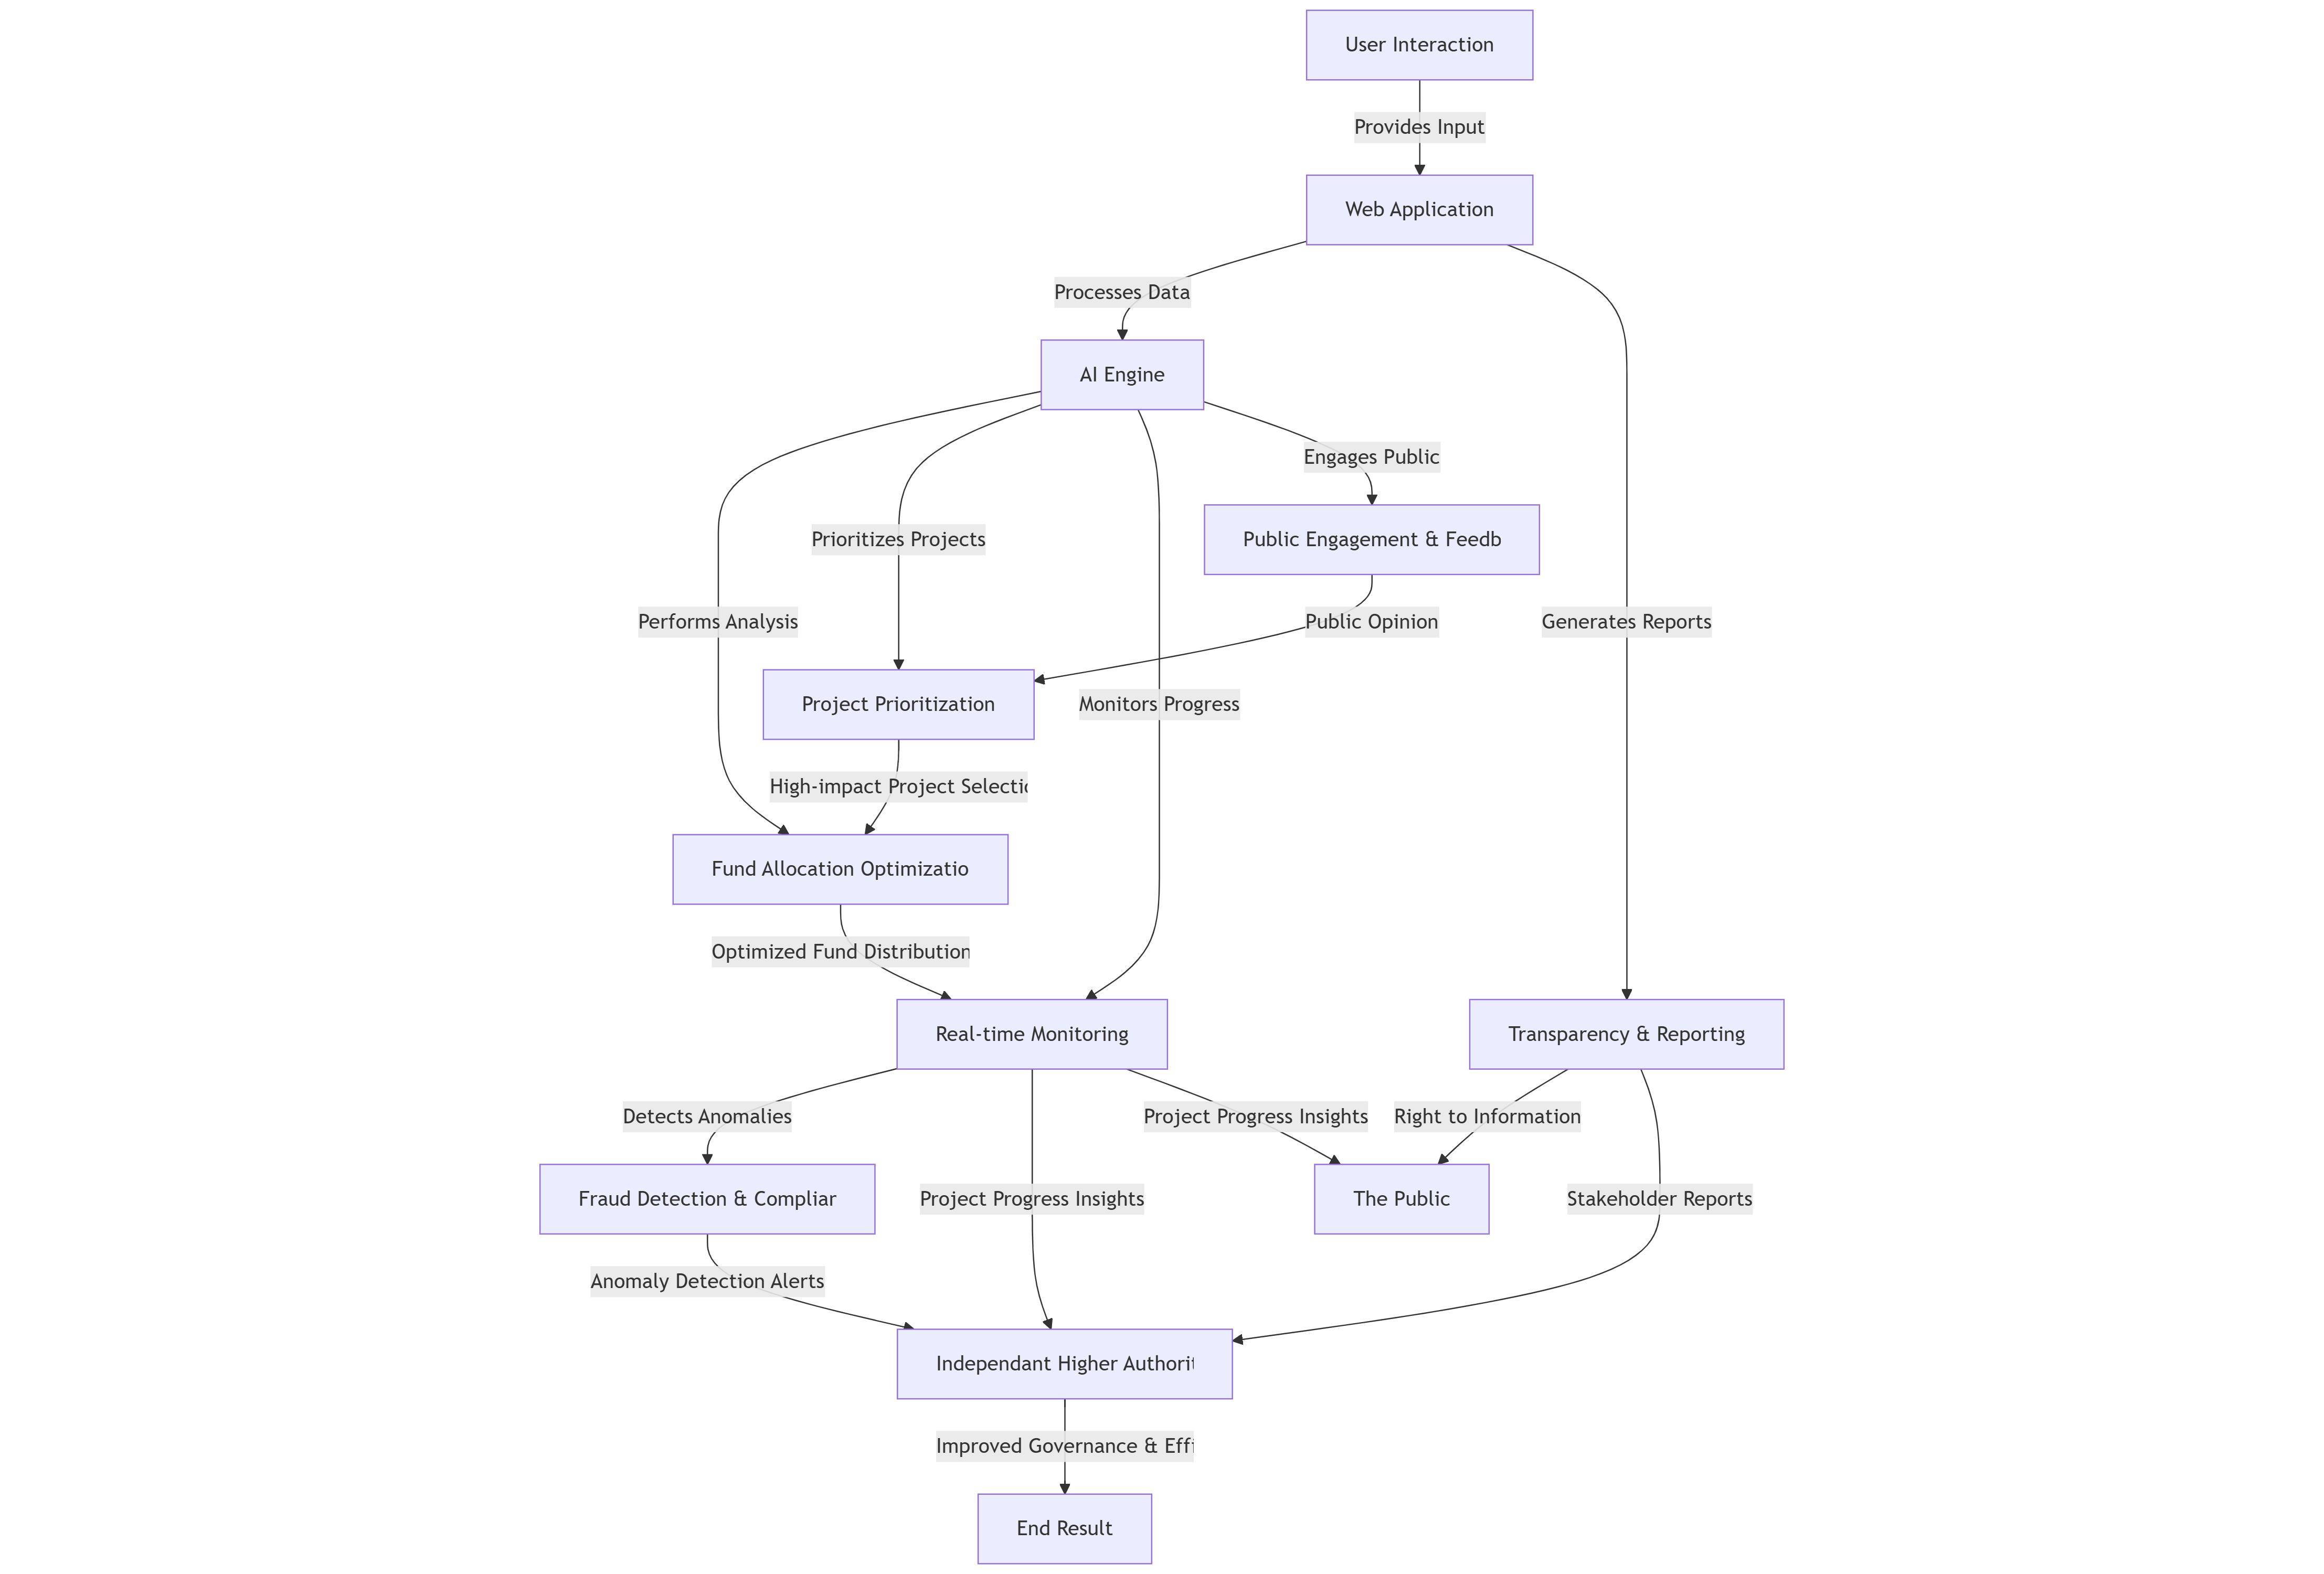
\includegraphics[width=1\linewidth]{mermaid-diagram-2025-02-13-134150.png}
    \label{fig:enter-label}
\end{itemize}



\end{document}

